%********************************************************************
% Appendix
%*******************************************************
% If problems with the headers: get headings in appendix etc. right
%\markboth{\spacedlowsmallcaps{Appendix}}{\spacedlowsmallcaps{Appendix}}
\chapter{Appendix}
%\section{On the inversion between dependent and independent variables}
%\label{appendix:a}
%Given n observations $(x_i,y_i)$ with $i=1,2,\dotsc,n$ in the plane, they can be linearly approximated by a straight line $y=\beta x+e$. After estimation we obtain the fitted value that is $\hat{y}$, then the residuals are computed as $(y_i - \hat{y}_i) = (y_i - \beta x_i - e)$ and the total squared residuals are $\sum_{i=1}^n (y_i-\beta x_i-e)^2$. We want to obtain the values of a and b such that the sum of squared residuals is minimized.
%It is important to note that $(y_i-\beta x_i-e)$ is the vertical distance of $(x_i,y_i)$ from the straight line.
%If dependent and independent variables are inverted and so data is approximated by $x=\beta y + e$ the squared sum of residuals become $\sum_{i=1}^n (x_i - \beta y_i - e)^2$ that is the horizontal distance from the straight line.
%The minimization of the residuals will led to different results if trivial results are ignored.

%\begin{figure}
 %   \centering
  %  \hspace*{-1.5cm}
   % \subfloat[\centering $y\sim x$]{{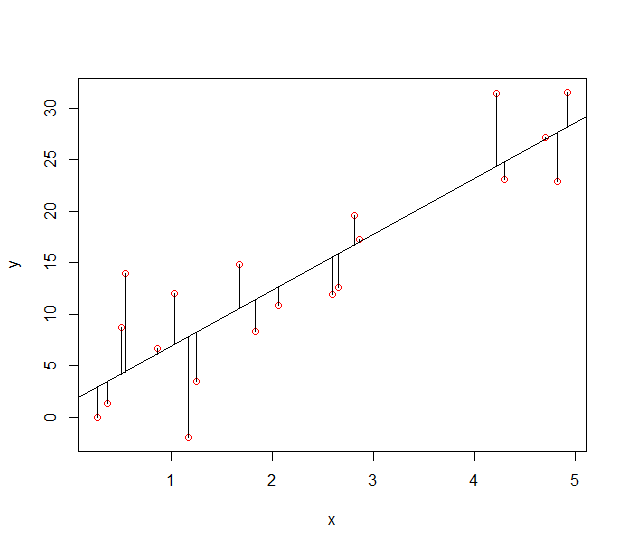
\includegraphics[width=8cm]{images/correct.png} }}%
    %\subfloat[\centering $x\sim y$]{{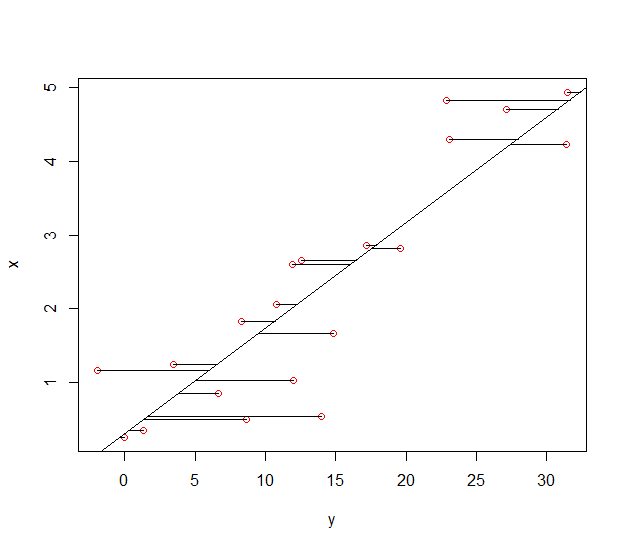
\includegraphics[width=8cm]{images/wrong.png} }}%
    %\caption{Inverting dependent with independent variable in linear regression}%
    %\label{fig:wrongvscorrect}
%\end{figure}
%In fact, looking at bivariate derivation of $\beta$ parameter we get in the first case:
%\begin{equation}
 %   b_{y\sim x}=\frac{cov(x,y)}{var(x)}
  %  \label{eq:true}
%\end{equation}
%While, in the second case
%\begin{equation}
 %   b_{x\sim y}=\frac{cov(x,y)}{var(y)}
  %  \label{eq:wrong}
%\end{equation}
%Note that \ref{eq:wrong} can be rewritten as:
%\begin{equation}
 %   b_{x\sim y}=\frac{cov(x,y)}{var(y)}=\frac{cov(x,y)}{var(y)}\cdot \frac{var(x)}{var(x)}=
  %  =\frac{cov(x,y)}{var(x)}\cdot \frac{var(x)}{var(y)}
   % \label{eq:wrong}
%\end{equation}
%That is the slope of $b_{y\sim x}$ times $\frac{var(x)}{var(y)}$. Thus, reversing dependent with independent will led to biased estimate of b.
\section{Panel data regression}
Panel regressions with different estimates of GDP growth at current prices, local unit currency at constant prices, local unit currency at current prices and purchasing power parity adjusted.
\begin{table}[h!]
\centering
\caption{Panel data regressions results}
\label{table:coefficients}
\resizebox{\linewidth}{!}{%
\begin{tabular}{lcccc} 
\hline
 & Current prices & LUC constant & LUC current & PPP \\ 
\hline
sum\_growth & $0.08^{**}$ & $0.08^{**}$ & $0.05$ & $0.06^{**}$ \\
 & $(0.03)$ & $(0.03)$ & $(0.08)$ & $(0.02)$ \\
factor(year)2013 & $-0.02^{**}$ & $-0.02^{**}$ & $-0.08^{***}$ & $-0.02^{**}$ \\
 & $(0.01)$ & $(0.01)$ & $(0.02)$ & $(0.01)$ \\
factor(year)2014 & $-0.01$ & $-0.01$ & $-0.08^{***}$ & $-0.01^*$ \\
 & $(0.00)$ & $(0.00)$ & $(0.02)$ & $(0.00)$ \\
factor(year)2015 & $-0.01^{**}$ & $-0.01^{**}$ & $-0.10^{***}$ & $-0.01^{**}$ \\
 & $(0.00)$ & $(0.00)$ & $(0.02)$ & $(0.00)$ \\
factor(year)2016 & $-0.01^*$ & $-0.01^*$ & $-0.08^{***}$ & $-0.01^{**}$ \\
 & $(0.00)$ & $(0.00)$ & $(0.02)$ & $(0.00)$ \\
factor(year)2018 & $-0.01^{***}$ & $-0.01^{***}$ & $-0.07^{***}$ & $-0.01^{***}$ \\
 & $(0.00)$ & $(0.00)$ & $(0.02)$ & $(0.00)$ \\
factor(year)2019 & $-0.02^{***}$ & $-0.02^{***}$ & $-0.07^{***}$ & $-0.02^{***}$ \\
 & $(0.00)$ & $(0.00)$ & $(0.02)$ & $(0.00)$ \\
factor(year)2020 & $-0.09^{***}$ & $-0.09^{***}$ & $-0.15^{***}$ & $-0.10^{***}$ \\
 & $(0.01)$ & $(0.01)$ & $(0.02)$ & $(0.01)$ \\ 
\hline
Num. obs. & $1605$ & $1607$ & $1629$ & $1523$ \\
Num. groups: country & $206$ & $207$ & $210$ & $193$ \\
R$^2$ (full model) & $0.47$ & $0.47$ & $0.38$ & $0.47$ \\
R$^2$ (proj model) & $0.33$ & $0.33$ & $0.05$ & $0.34$ \\
Adj. R$^2$ (full model) & $0.38$ & $0.38$ & $0.28$ & $0.39$ \\
Adj. R$^2$ (proj model) & $0.32$ & $0.32$ & $0.05$ & $0.34$ \\ 
\hline
\multicolumn{5}{l}{$^{***}p<0.001$; $^{**}p<0.01$; $^{*}p<0.05$}
\end{tabular}
}
\end{table}

\cleardoublepage


\section{Country data quality groups}


\begin{table}[h!]
\fontsize{11}{9}\selectfont
\centering
\caption{Data quality country groups}
\label{table:qualitygroups}
\resizebox{\linewidth}{!}{%
\begin{tabular}{|>{\hspace{0pt}}p{0.181\linewidth}|>{\hspace{0pt}}p{0.258\linewidth}|>{\hspace{0pt}}p{0.356\linewidth}|>{\hspace{0pt}}p{0.142\linewidth}|} 
\hline
\multicolumn{1}{|>{\centering\hspace{0pt}}m{0.181\linewidth}|}{Group A} & \multicolumn{1}{>{\centering\hspace{0pt}}m{0.258\linewidth}|}{Group B} & \multicolumn{1}{>{\centering\hspace{0pt}}m{0.356\linewidth}|}{Group C} & \multicolumn{1}{>{\centering\arraybackslash\hspace{0pt}}m{0.142\linewidth}|}{Group D} \\ 
\hline
\vcell{Armenia, Australia, Austria, Canada, Switzerland, Chile, Czechia, Germany, Denmark, Spain, Estonia, Finland, France, United Kingdom, Greece, Hungary, Ireland, Italy, Japan, South Korea, Lithuania, Latvia, Mexico, Netherlands, Norway, New Zealand, Poland, Portugal, Slovakia, Slovenia, Sweden, Turkey, United States} & \vcell{Albania, Argentina, Azerbaijan, Belgium, Bulgaria, Belarus, Bolivia, Brazil, Colombia, Costa Rica, Cyprus, Dominican Republic, Ecuador, Egypt, Georgia, Guatemala, Honduras, Croatia, Indonesia, India, Iceland, Israel, Kazakhstan, Kyrgyzstan, Sri Lanka, Luxembourg, Moldova, North Macedonia, Malta, Montenegro, Mongolia, Mauritius, Malaysia, Peru, Philippines, Russia, Rwanda, Singapore, El Salvador, Serbia, Thailand, Tunisia, Tanzania, Uganda, Ukraine, Uruguay, Vietnam, South Africa} & \vcell{Afghanistan, Angola, United Arab Emirates, Burundi, Benin, Burkina Faso, Bangladesh, Bahrain, Bahamas, Bosnia  Herzegovina, Belize, Bhutan, Botswana, China, Côte d’Ivoire, Cameroon, Cape Verde, Algeria, Ethiopia, Fiji, Ghana, Guinea, Gambia, Iran, Jamaica, Jordan, Kenya, Cambodia, Kuwait, Laos, Lebanon, Liberia, St. Lucia, Lesotho, Morocco, Madagascar, Maldives, Mali, Myanmar (Burma), Mozambique, Mauritania, Malawi, Namibia, Niger, Nigeria, Nicaragua, Nepal, Oman, Pakistan, Panama, Paraguay, Qatar, Saudi Arabia, Senegal, Sierra Leone, São Tomé  Príncipe, Suriname, Eswatini, Togo, Tajikistan, Trinidad  Tobago, Uzbekistan, St. Vincent  Grenadines, Venezuela, Samoa, Zambia, Zimbabwe} & \vcell{Congo - Brazzaville, Djibouti, Micronesia (Federated States of), Gabon, Guinea-Bissau, Guyana, Haiti, Iraq, Kiribati, Libya, Marshall Islands, Papua New Guinea, Sudan, Solomon Islands, South Sudan, Chad, Turkmenistan, Vanuatu, Yemen} \\[-\rowheight]
\printcelltop & \printcelltop & \printcelltop & \printcelltop \\
\hline
\end{tabular}
}
\end{table}
\cleardoublepage
\section{Extreme values removal results}
\begin{table}[h!]
\fontsize{11}{9}\selectfont
\centering
\caption{Percentage differences after removing raster values greater than 5\%}
\label{table:differences}
\resizebox{\linewidth}{!}{%
\begin{tabular}{>{\hspace{0pt}}m{0.088\linewidth}>{\hspace{0pt}}m{0.121\linewidth}>{\hspace{0pt}}m{0.098\linewidth}>{\hspace{0pt}}m{0.09\linewidth}>{\hspace{0pt}}m{0.121\linewidth}>{\hspace{0pt}}m{0.098\linewidth}>{\hspace{0pt}}m{0.09\linewidth}>{\hspace{0pt}}m{0.121\linewidth}>{\hspace{0pt}}m{0.098\linewidth}} 
\hline
Country & Year & \% diff & Country & Year & \% diff & Country & Year & \% diff \\ 
\hline
\rowcolor[rgb]{0.902,0.902,0.902} COG & $2013$ & $13$ & IRQ & $2021$ & $27$ & NLD & $2021$ & $12$ \\
COG & $2019$ & $11$ & KAZ & $2013$ & $27$ & OMN & $2013$ & $8$ \\
\rowcolor[rgb]{0.902,0.902,0.902} COG & $2020$ & $16$ & KAZ & $2014$ & $37$ & OMN & $2014$ & $8$ \\
COG & $2021$ & $12$ & KAZ & $2015$ & $33$ & OMN & $2015$ & $6$ \\
\rowcolor[rgb]{0.902,0.902,0.902} DZA & $2013$ & $18$ & KAZ & $2016$ & $22$ & OMN & $2016$ & $7$ \\
DZA & $2014$ & $17$ & KAZ & $2018$ & $10$ & OMN & $2018$ & $5$ \\
\rowcolor[rgb]{0.902,0.902,0.902} DZA & $2015$ & $15$ & KAZ & $2019$ & $8$ & OMN & $2019$ & $5$ \\
DZA & $2016$ & $17$ & KAZ & $2020$ & $6$ & OMN & $2020$ & $5$ \\
\rowcolor[rgb]{0.902,0.902,0.902} DZA & $2018$ & $13$ & KAZ & $2021$ & $6$ & PNG & $2014$ & $11$ \\
DZA & $2019$ & $14$ & KWT & $2013$ & $7$ & QAT & $2013$ & $5$ \\
\rowcolor[rgb]{0.902,0.902,0.902} DZA & $2020$ & $14$ & KWT & $2014$ & $11$ & RUS & $2013$ & $12$ \\
DZA & $2021$ & $8$ & KWT & $2015$ & $8$ & RUS & $2014$ & $11$ \\
\rowcolor[rgb]{0.902,0.902,0.902} EST & $2014$ & $6$ & KWT & $2016$ & $8$ & RUS & $2015$ & $9$ \\
EST & $2015$ & $7$ & LBY & $2013$ & $10$ & RUS & $2016$ & $11$ \\
\rowcolor[rgb]{0.902,0.902,0.902} EST & $2016$ & $6$ & LBY & $2014$ & $7$ & RUS & $2018$ & $16$ \\
EST & $2021$ & $6$ & LBY & $2015$ & $8$ & RUS & $2019$ & $17$ \\
\rowcolor[rgb]{0.902,0.902,0.902} FIN & $2015$ & $6$ & LBY & $2016$ & $6$ & RUS & $2020$ & $20$ \\
FIN & $2016$ & $6$ & LBY & $2018$ & $10$ & RUS & $2021$ & $18$ \\
\rowcolor[rgb]{0.902,0.902,0.902} FIN & $2018$ & $8$ & LBY & $2019$ & $14$ & TCD & $2013$ & $24$ \\
FIN & $2019$ & $7$ & LBY & $2021$ & $15$ & TCD & $2014$ & $17$ \\
\rowcolor[rgb]{0.902,0.902,0.902} FIN & $2020$ & $12$ & MEX & $2021$ & $6$ & TCD & $2015$ & $14$ \\
FIN & $2021$ & $10$ & NER & $2014$ & $6$ & TCD & $2016$ & $16$ \\
\rowcolor[rgb]{0.902,0.902,0.902} GAB & $2021$ & $5$ & NGA & $2013$ & $10$ & TCD & $2018$ & $6$ \\
IRN & $2013$ & $12$ & NGA & $2014$ & $8$ & TKM & $2013$ & $20$ \\
\rowcolor[rgb]{0.902,0.902,0.902} IRN & $2014$ & $13$ & NGA & $2015$ & $12$ & TKM & $2014$ & $14$ \\
IRN & $2015$ & $13$ & NGA & $2016$ & $7$ & TKM & $2015$ & $12$ \\
\rowcolor[rgb]{0.902,0.902,0.902} IRN & $2016$ & $17$ & NGA & $2018$ & $13$ & TKM & $2016$ & $14$ \\
IRN & $2018$ & $15$ & NGA & $2019$ & $9$ & TKM & $2018$ & $10$ \\
\rowcolor[rgb]{0.902,0.902,0.902} IRN & $2019$ & $11$ & NGA & $2020$ & $6$ & TKM & $2019$ & $9$ \\
IRN & $2020$ & $9$ & NGA & $2021$ & $7$ & UKR & $2013$ & $5$ \\
\rowcolor[rgb]{0.902,0.902,0.902} IRQ & $2013$ & $41$ & NLD & $2013$ & $14$ & UKR & $2014$ & $6$ \\
IRQ & $2014$ & $41$ & NLD & $2014$ & $17$ & UKR & $2015$ & $7$ \\
\rowcolor[rgb]{0.902,0.902,0.902} IRQ & $2015$ & $43$ & NLD & $2015$ & $17$ & UKR & $2016$ & $7$ \\
IRQ & $2016$ & $44$ & NLD & $2016$ & $16$ & UKR & $2018$ & $6$ \\
\rowcolor[rgb]{0.902,0.902,0.902} IRQ & $2018$ & $32$ & NLD & $2018$ & $16$ & VUT & $2016$ & $25$ \\
IRQ & $2019$ & $31$ & NLD & $2019$ & $14$ &  &  &  \\
\rowcolor[rgb]{0.902,0.902,0.902} IRQ & $2020$ & $27$ & NLD & $2020$ & $13$ &  &  &  \\
\hline
\end{tabular}
}
\end{table}